\documentclass[12pt, a4paper, oneside]{ctexart}
\usepackage{amsmath, amsthm, amssymb, bm, color, graphicx, geometry, hyperref, mathrsfs,extarrows, braket, booktabs, array}

\linespread{1.5}
%\geometry{left=2.54cm,right=2.54cm,top=3.18cm,bottom=3.18cm}
\geometry{left=1.84cm,right=1.84cm,top=2.18cm,bottom=2.18cm}
\newenvironment{problem}{\par\noindent\textbf{题目. }}{\bigskip\par}
\newenvironment{solution}{\par\noindent\textbf{解答. }}{\bigskip\par}
\newenvironment{note}{\par\noindent\textbf{注记. }}{\bigskip\par}

% 基本信息
\newcommand{\RQ}{\today} % 日期
\newcommand{\km}{实变函数} % 科目
\newcommand{\bj}{强基数学002} % 班级
\newcommand{\xm}{吴天阳} % 姓名
\newcommand{\xh}{2204210460} % 学号
\newcommand{\XH}{59} % 序号

\begin{document}

%\pagestyle{empty}
\pagestyle{plain}
\vspace*{-15ex}
\centerline{\begin{tabular}{*6{c}}
    \parbox[t]{0.25\linewidth}{\begin{center}\textbf{日期}\\ \large \textcolor{blue}{\RQ}\end{center}} 
    & \parbox[t]{0.15\linewidth}{\begin{center}\textbf{科目}\\ \large \textcolor{blue}{\km}\end{center}}
    & \parbox[t]{0.2\linewidth}{\begin{center}\textbf{班级}\\ \large \textcolor{blue}{\bj}\end{center}}
    & \parbox[t]{0.1\linewidth}{\begin{center}\textbf{姓名}\\ \large \textcolor{blue}{\xm}\end{center}}
    & \parbox[t]{0.15\linewidth}{\begin{center}\textbf{学号}\\ \large \textcolor{blue}{\xh}\end{center}}
    & \parbox[t]{0.1\linewidth}{\begin{center}\textbf{序号}\\ \large \textcolor{blue}{\XH}\end{center}} \\ \hline
\end{tabular}}
\vspace*{4ex}

\paragraph{习题 1.4}
\paragraph{5.}记$A'=A^{(1)},(A^{(1)})'=A^{(2)},\cdots,(A^{(n)})'=A^{(n+1)},\cdots$.试作一集$A$,使$A^{(n)}(n=1,2,\cdots)$彼此互异.
\def\disp{\displaystyle}
\begin{solution}
    设$A_i$为直线上的一孤立点集,将$A_i$中的元素从小到大排成一行,即
    \begin{equation*}
      A_i = \{x_1,x_2,\cdots,x_{j-1},x_j,x_{j+1},\cdots\}
    \end{equation*}
    记$d_j = x_{j+1}-x_j$即为第$j$个间距的大小.于是可以做出如下构造
    \begin{equation*}
        A_{i+1} = \left\{x_j+\frac{d_j}{k}:x_j\in A_i,\ k=2,3,\cdots\right\}
    \end{equation*}
    下证$A_i\cap A_{i+1} = \varnothing$且$(A_{i+1})' = A_i$.

    反设$\exists x_j\in A_i\cap A_{i+1}$,则由$A_{i+1}$的定义可知,\ $ x_j=x_{j-1}+\frac{d_j}{k}=x_{j-1}+\frac{1}{k}(x_j-x_{j-1})$,则$k=1$,与$k\geqslant 2$矛盾,则$A_i\cap A_{i+1} = \varnothing$.

    对于$\forall x_j\in A_i$,存在$A_{i+1}$中的点列$\left\{x_j+\frac{d_j}{2},x_j+\frac{d_j}{3},\cdots,x_j+\frac{d_j}{n},\cdots\right\}$收敛于$x_j$,所以$A_i\subset (A_{i+1})'$.相应的,对于$\forall a\in (A_{i+1})'$,一定存在$j$,使得$x_{j-1}\leqslant a < x_j$,由于$A_{i+1}$在区间$[x_{j-1},x_j)$中仅有唯一一个收敛子列$\left\{x_j+\frac{d_j}{2},x_j+\frac{d_j}{3},\cdots,x_j+\frac{d_j}{n},\cdots\right\}$收敛于$x_j$,所以$a = x_j\in A_i$,于是$(A_{i+1})' \subset A_i$.综上$(A_{i+1})' = A_i$.

    取$ A_1 = \{0, \frac{1}{2},\frac{1}{3},\frac{1}{4},\cdots\}$,则可根据上述构造方法得到一孤立点集列$\{A_1,A_2,\cdots, A_n,\cdots\}$,对于$\forall i = 1,2,\cdots$,满足$(A_{i+1})'=A_i$且$A_{i+1}\cap A_i = \varnothing$,于是当$i\rightarrow \infty$时,取$A = A_{\infty}$,满足题目要求.

    更严谨地,由于$A_i\subset [0,1)$,记$A_i+i = \{a+i:a\in A_i\}$,则$\{A_i+i\}\subset [i, i+1)$,所以$\{A_i+i\}$是一列两两不交的集列,取$\disp A = \bigcup_{i=1}^{\infty}(A_i+i)$即可.
\end{solution}
\paragraph{6.}证明直线上的孤立点集必是有限集或可列集.
\begin{proof}
    设$A$为直线上的孤立点集,由孤立点集的定义,不妨令
    \begin{equation*}
        A = \{x_1,x_2,\cdots,x_n,\cdots\}
    \end{equation*}
    其中$0 < x_1 < x_2 < \cdots < x_n<\cdots$,令$x_0 = 0$,对于$\forall i = 1,2,\cdots$,若$x_i$为无理点,取$x_i'$为$(x_{i-1},x_i)$中的一个有理点;若$x_i$为有理点,取$x_i' = x_i$,于是有
    \begin{equation*}
        B = \{x_1', x_2', \cdots, x_n', \cdots\}
    \end{equation*}
    与$A$一一对应,由于$B\subset \mathbb{Q}$,则$B$为至多可列集,所以$A$也为至多可列集.
\end{proof}
\paragraph{7.}证明每个闭集必是可列个开集的通集,每个开集可以表示成可列个闭集的和集.
\begin{proof}
    设$F$为闭集,令$\disp G_n = \bigcup_{x\in F}(x-\frac{1}{n}, x+\frac{1}{n})$,则$\disp F\subset \bigcap_{n=1}^{\infty}G_n$.对于$\disp \forall x\in\bigcap_{n=1}^{\infty}G_n$,对于每个$n = 1,2,\cdots$,一定$\exists x_n\in F$,使得$\disp x\in \left(x_n-\frac{1}{n}, x_n + \frac{1}{n}\right)$,则存在$F$的点列$\{x_n\}$使得$\disp\lim_{n\rightarrow \infty}x_n = x$,由于$F'\subset F$,则$x\in F$,于是$\disp \bigcap_{n=1}^{\infty}G_n\subset F$.综上,$\ \disp F=\bigcap_{n=1}^{\infty}G_n$.

    设$G$为开集,不妨令$G$的构成区间为$\{(a_i,b_i):i=1,2,\cdots\}$,根据开集的性质可知$(a_i,b_i)\cap(a_j,b_j) = \varnothing,\ (i\neq j)$.如下定义$a_i',\ b_i'$:
    \begin{equation*}
        a_i' = 
        \begin{cases}
            a_i+\frac{1}{n},&\quad a_i\neq -\infty,\\
            -n,&\quad a_i = -\infty.
        \end{cases}\qquad
        b_i' = 
        \begin{cases}
            b_i-\frac{1}{n},&\quad b_i\neq \infty,\\
            n,&\quad b_i=\infty.
        \end{cases}
    \end{equation*}
    设$\disp F_n = \bigcup_{i=1}^{\infty}[a_i', b_i']$,则$\disp \bigcup_{n=1}^{\infty}F_n\subset G$.对于$\forall x\in G$,一定$\exists i$使得$x\in(a_i,b_i)$,存在一个尽可能大的$N$,使得$\disp \forall n\geqslant N$,有$\disp x\in[a_i',b_i']\in \bigcup_{n=1}^{\infty}F_n$,则$\disp G\subset \bigcup_{n=1}^{\infty}F_n$.综上,$\ \disp G= \bigcup_{n=1}^{\infty}F_n$.
\end{proof}
\paragraph{10.}证明直线上闭集全体所成的集的势是$\aleph$,直线上完全集全体所成的集的势也是$\aleph$.
\def\o{\overline}
\begin{proof}
    设直线上开集全体所成之集为$A$,闭集全体所成之集为$B$,完全集所成之集为$S$.
    
    令$G$为开集,不妨令$G$的构成区间为$\{(a_i,b_i):i=1,2,\cdots\}$,若$a_i,b_i$均为无理数,则存在有理数列$\left\{\left(\frac{[na_i]+1}{n},\frac{[nb_i]}{n}\right)\right\}$收敛于$(a_i,b_i)$,若$a_i,b_i$中存在无限点,则只考虑有理点趋于有限点一端.由于有理点全体的基数为$\aleph_0$,所以$\o{\o{A}} = 2^{\aleph_0} = \aleph$.又由于闭集与开集一一对应(互为余集),所以$\o{\o{B}} = \o{\o{A}} = \aleph$.

    任一完全集都是自密闭集,所以$S\subset B$,由于将开集的构成区间都加上端点,可以构成一完全集$S'\subset S$,而且$A$可以与$S'$一一对应,所以\begin{equation*}
        \aleph = \o{\o{A}} = \o{\o{S'}} \leqslant  \o{\o{S}}\leqslant \o{\o{B}} = \aleph
    \end{equation*}
    综上可知,\ $ \o{\o{S}} = \aleph$.
\end{proof}
\paragraph{15. 定义 1.4.14}设$A$是直线上点集,\ $x$是直线上的一点,如果在$x$的任何环境中总含有$A$中不可列无限的点,那么称$x$是$A$的\textbf{凝聚点}.

证明: (i) 对任何不可列无限集$A$,必有凝聚点,而且在$A$中必有一个点是$A$的凝聚点.

(ii) 如果$x$是$A$的凝聚点,那么$x$是$A$的凝聚点的极限点.

(iii) 直线上闭集$F$的势除了有限、可列外必为$\aleph$.
\begin{proof}
    (i) 由于$A$为不可列无限集,则存在$-\infty < a_1 < b_1 < \infty$,使得$(a_1,b_1)\cap A$为不可列无限集,将开区间$(a_1,b_1)$分为两半$\disp \left(a_1,\frac{a_1+b_1}{2}\right),\ \left(\frac{a_1+b_1}{2},b_1\right)$,则二者中至少有一个与$A$交集为不可列无限集,记为$(a_2,b_2)$.依此类推,可得一开区间列$\{(a_n,b_n)\}$,满足$\disp b_n-a_n\leqslant \frac{b_1-a_1}{2^{n-1}}$,且$(a_n,b_n)\cap A$为不可列无限集,由区间套定理可知,存在唯一的$x_0\in E^1$,使得$x_0\in (a_n,b_n)\ (n=1,2,\cdots)$,则$x_0$为$A$的凝聚点.

    反设$A$中没有凝聚点,则$\forall x \in A$,存在$x$的邻域$(a_x,b_x)$,使得$(a,b)\cap A$为至多可列集,不妨令$a_x,b_x$均为有限数,则$\disp A=\bigcup_{x\in A}((a_x,b_x)\cap A)$,则$A$为至多可列集,与$A$为不可列无限集矛盾.
    
    (ii) 记$S$为凝聚点全体,只需证$S$为自密集,令$x$为$A$的凝聚点,下证$x \in S'$.对于$n = 1,2,\cdots$有$ \left(x-\frac{1}{n},x+\frac{1}{n}\right)\cap A$,为不可列无限集,则$(x-\frac{1}{n}, x)\cap A$和$(x, x+\frac{1}{n})\cap A$中至少有一个是不可列无限集,有$(i)$可知,不可列无限集中必存在凝聚点,记为$x_n$,则$x_n\in(x-\frac{1}{n},x+\frac{1}{n})-\{x\}$且$x_n\in S$,根据上述方法,可以构造出$S$中一列收敛点列$\{x_n\}$且$\disp\lim_{n\rightarrow \infty}x_n=x$,则$x\in S'$.

    (iii) 设$F$为非空闭集,则$F$为不可列无限集,于是存在两个凝聚点$a_1,a_2$,由闭集的性质,存在$a_1,a_2$的邻域包含于$F$,且也是不可列无限点集,于是可以找到$a_{11},a_{12}$属于$a_{1}$的邻域,$\ a_{21}, a_{22}$属于$a_{2}$的邻域,以此类推,可得$F$的一子集$F' = \{a_1, a_2, a_{11},a_{12}, a_{21}, a_{22},\cdots\}$,且$\o{\o{F'}} = 2^{\aleph_0} = \aleph$,又由于全体闭集的势为$\aleph$,所以$\aleph = \o{\o{F'}}\leqslant \o{\o{F}} \leqslant \aleph$,故$\o{\o{F}} = \aleph$.

\end{proof}

\paragraph{18.}直线上的完全集$A$,如果具有如下性质:任何两个余区间之间必至少夹有一个余区间.问是否$A$必是疏朗的.
\begin{proof}
    不一定, 设$C$为$(0,1)$上的康托集, 取$A = (-\infty, 0]\cup C\cup [1,\infty)$, 由于康托集的性质, 两个余区间之间必至少夹有一个余区间, 但$(-\infty,0]$不是疏朗的, 则$A$不是疏朗的.
\end{proof}
\paragraph{22.}证明无理数全体不能表示成可列个闭集的和集.
\begin{proof}
    反设$\mathbb{Q}^c$可以表示成可列个闭集的和集,即$\disp \mathbb{Q}^c = \bigcup_{i = 1}^{\infty}F_{i}$,记$\mathbb{Q} = \{x_1,x_2,\cdots\} = \bigcup_{j=1}^{\infty}x_j$,则$\disp\mathbb{R} = \left(\bigcup_{i=1}^{\infty}F_i\right)\cup\left(\bigcup_{j=1}^{\infty}x_j\right)$,由Baire定理可知,$\mathbb{R}$没有内点,矛盾.原命题得证.
\end{proof}

\iffalse
% 图片模板
\centerline{
    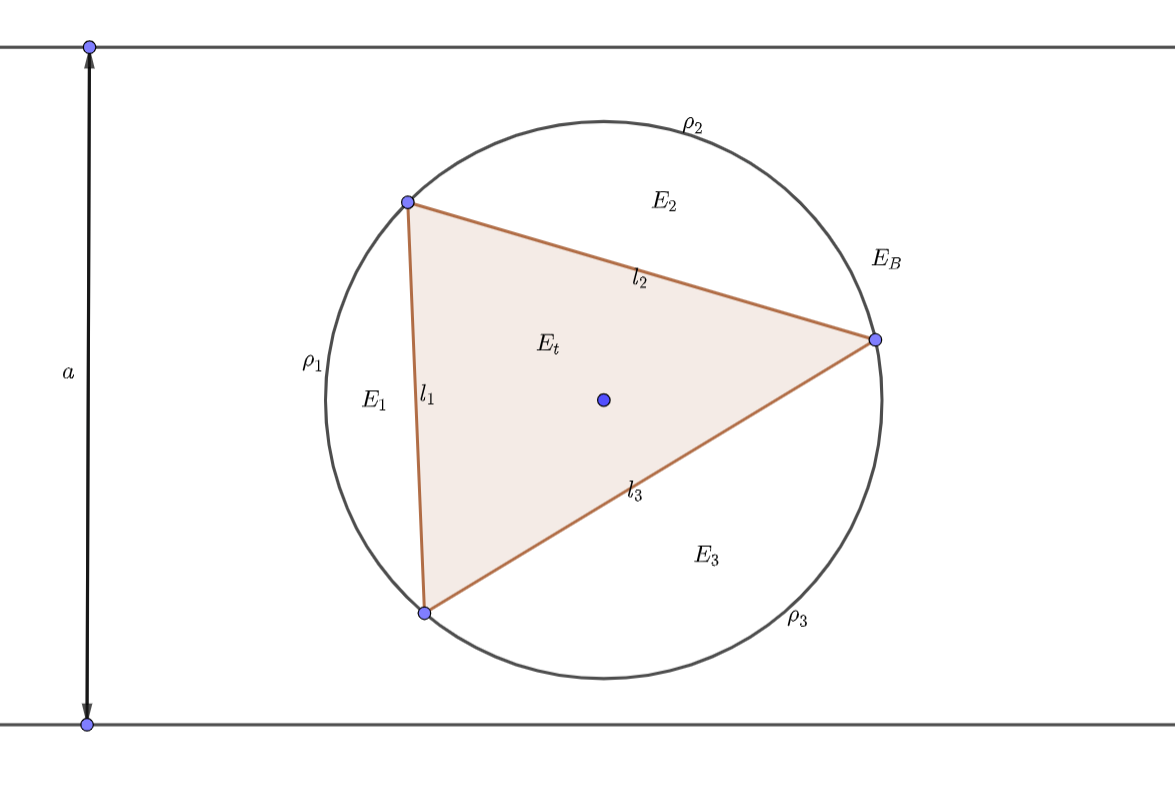
\includegraphics[width=0.8\textwidth]{figure.png}
}
\fi
\iffalse
% 表格模板
\renewcommand\arraystretch{0.8} % 设置表格高度为原来的0.8倍
\begin{table}[!htbp] % table标准
    \centering % 表格居中
    \begin{tabular}{p{1cm}<{\centering}p{1cm}<{\centering}p{3cm}<{\centering}p{5cm}<{\centering}} % 设置表格宽度
    %\begin{tabular}{cccc}
        \toprule
        $x_i$ & $f[x_1]$ & $f[x_i,x_{i+1}]$ & $f[x_i,x_{i+1},x_{i+2}]$ \\
        \midrule
        $x_0$ & $f(x_0)$ &                  &                          \\
        $x_0$ & $f(x_0)$ & $f'(x_0)$        &                          \\
        $x_0$ & $f(x_1)$ & $\frac{f(x_1)-f(x_0)}{x_1-x_0}$ & $\frac{f(x_1)-f(x_0)}{(x_1-x_0)^2}-\frac{f'(x_0)}{x_1-x_0}$\\
        \bottomrule
    \end{tabular}
\end{table}

\def\Log{\text{Log}} % 一个简单的宏定义
$\Log$ % 调用方法
\fi

\end{document}